\documentclass[10pt,a4paper]{article}

\usepackage[brazilian]{babel}
\usepackage[T1]{fontenc}
\usepackage[utf8]{inputenc}
\usepackage{lmodern}
\usepackage{microtype}
\usepackage[a4paper,top=1.8cm,bottom=1.8cm,left=2.1cm,right=2.1cm]{geometry}
\usepackage{graphicx}
\usepackage{booktabs}
\usepackage{tabularx}
\usepackage{amsmath,amssymb}
\usepackage{enumitem}
\usepackage{caption}
\usepackage{subcaption}
\usepackage{xcolor}
\usepackage{listings}
\usepackage{csquotes}
\usepackage{fancyhdr}
\usepackage[hidelinks]{hyperref}
\usepackage[backend=biber,style=numeric,sorting=none]{biblatex}

\addbibresource{references.bib}
\graphicspath{{../figuras/}}

\definecolor{codegray}{RGB}{245,245,245}
\lstset{
  basicstyle=\ttfamily\small,
  backgroundcolor=\color{codegray},
  frame=single,
  columns=fullflexible,
  keepspaces=true,
  showstringspaces=false,
  breaklines=true,
  inputencoding=utf8,
  extendedchars=true,
  literate=
    {á}{{\'a}}1 {à}{{\`a}}1 {ã}{{\~a}}1 {â}{{\^a}}1
    {é}{{\'e}}1 {ê}{{\^e}}1 {í}{{\'i}}1
    {ó}{{\'o}}1 {õ}{{\~o}}1 {ô}{{\^o}}1
    {ú}{{\'u}}1 {ç}{{\c c}}1
    {Á}{{\'A}}1 {À}{{\`A}}1 {Ã}{{\~A}}1 {Â}{{\^A}}1
    {É}{{\'E}}1 {Ê}{{\^E}}1 {Í}{{\'I}}1
    {Ó}{{\'O}}1 {Õ}{{\~O}}1 {Ô}{{\^O}}1
    {Ú}{{\'U}}1 {Ç}{{\c C}}1
}

\setlist{nosep,leftmargin=1.4em}
\captionsetup{font=small,labelfont=bf}
\setlength{\parindent}{1.2em}
\setlength{\parskip}{0.15em}
\setlength{\emergencystretch}{2em}
\setlength{\tabcolsep}{5pt}
\renewcommand{\arraystretch}{1.08}

\pagestyle{fancy}
\fancyhf{}
\lhead{Rede Intelectual da DBpedia}
\rhead{MC859}
\cfoot{\thepage}
\setlength{\headheight}{13pt}

\hypersetup{
  pdftitle={Rede Intelectual da DBpedia},
  pdfauthor={Raphael Salles Vitor de Souza e Lucas Félix},
  pdfsubject={Relatório final de MC859},
  colorlinks=true,
  linkcolor=black,
  citecolor=black,
  urlcolor=blue
}

\title{\vspace{-1.5cm}\textbf{Rede Intelectual da DBpedia}\\[0.25em]
  \large Aplicação de PageRank e análise estrutural em um grafo de conhecimento}
\author{Raphael Salles Vitor de Souza (RA 223641) \and Lucas Félix (RA 247064)}
\date{MC859 --- Projeto em Teoria da Computação\\
  Prof. Ruben Interian Kovaliova --- Universidade Estadual de Campinas\\
  22 de junho de 2026}

\begin{document}

\maketitle
\vspace{-1.2em}
\begin{center}
  \fbox{\parbox{0.92\linewidth}{\centering
    \textbf{Implementação pública:}
    \url{https://github.com/RaphaelSVSouza/mc859-dbpedia-intellectual-network}}}
\end{center}
\vspace{0.4em}

\section{Introdução}

Grafos de conhecimento representam entidades como vértices e relações semânticas como arestas. Essa estrutura permite estudar não apenas os atributos isolados de uma entidade, mas também sua posição em uma rede de relações. A DBpedia é especialmente adequada a esse tipo de análise porque extrai informação estruturada da Wikipédia e a disponibiliza como dados ligados, reunindo entidades de diferentes domínios em uma base de conhecimento aberta~\cite{dbpedia-about}.

Este trabalho construiu uma rede intelectual a partir da DBpedia, concentrando-se em relações de influência, orientação acadêmica, formação, áreas de atuação, obras, religião e ideologia. A hipótese investigada é que a estrutura dessas relações contém sinais capazes de distinguir entidades relevantes e de recuperar parte da organização semântica presente no domínio. Em vez de considerar toda a DBpedia, foi produzido um subgrafo temático direcionado, adequado à execução de algoritmos de centralidade em hardware acadêmico convencional.

A análise foi dividida em três partes. Primeiro, estudaram-se propriedades estruturais do grafo, como distribuição de graus e componentes fortemente conexas. Em seguida, aplicou-se PageRank para produzir rankings globais em três projeções distintas: o grafo completo, uma projeção voltada a pessoas e uma projeção institucional. Por fim, o Personalized PageRank foi empregado em um experimento de predição de arestas.

\subsection{Objetivo geral}

Construir e analisar um grafo de conhecimento direcionado, derivado da DBpedia, para investigar em que medida sua topologia permite identificar entidades intelectualmente relevantes e recuperar relações ocultadas do grafo.

\subsection{Objetivos específicos}

\begin{itemize}
  \item extrair do dump da DBpedia um subconjunto de relações associadas à rede intelectual;
  \item normalizar a orientação semântica de relações inversas e eliminar triplas duplicadas;
  \item serializar o grafo nos formatos N-Triples, GEXF e GraphML;
  \item instanciar o grafo no Neo4j e projetá-lo com o Graph Data Science;
  \item caracterizar sua estrutura por métricas de grau e conectividade;
  \item comparar variantes do PageRank voltadas a pessoas e instituições;
  \item avaliar os rankings obtidos por meio de referências externas;
  \item avaliar o Personalized PageRank como método de predição de ligações.
\end{itemize}

\section{Aquisição e preparação dos dados}

\subsection{Fonte dos dados}

A coleta utilizou o arquivo \texttt{mappingbased-objects\_lang=en.ttl.bz2}, correspondente ao componente \textit{mapping-based objects} em inglês da DBpedia, no snapshot de 1º de dezembro de 2022~\cite{dbpedia-dump}. Esse dump contém triplas RDF extraídas principalmente das infocaixas da Wikipédia. Cada registro segue a forma $\langle s,p,o\rangle$, na qual $s$ é o recurso de origem, $p$ é o predicado e $o$ é outro recurso identificado por URI.

O dump utilizado continha 22.791.171 triplas. Como o objetivo não era reproduzir toda a DBpedia, foram selecionados 11 predicados relacionados à circulação de influência e à caracterização intelectual: \texttt{influencedBy}, \texttt{influenced}, \texttt{doctoralAdvisor}, \texttt{doctoralStudent}, \texttt{academicAdvisor}, \texttt{almaMater}, \texttt{knownFor}, \texttt{notableWork}, \texttt{field}, \texttt{religion} e \texttt{ideology}.

A filtragem foi feita por correspondência literal com \texttt{grep -F}, utilizando a lista versionada em \texttt{pipeline/preds.txt}. Esse procedimento reduziu o conjunto para 432.975 triplas.

\subsection{Reorientação das relações}

Predicados inversos podem representar a mesma relação com direções opostas. Para estabelecer uma convenção única, três relações foram reescritas:

\begin{align*}
\operatorname{influencedBy}(A,B)&\longrightarrow\operatorname{influenced}(B,A),\\
\operatorname{doctoralAdvisor}(A,B)&\longrightarrow\operatorname{doctoralStudent}(B,A),\\
\operatorname{academicAdvisor}(A,B)&\longrightarrow\operatorname{academicStudent}(B,A).
\end{align*}

Assim, as arestas de influência e orientação passaram a apontar do influenciador ou orientador para a pessoa influenciada ou orientada. A transformação foi implementada com \texttt{awk}, trocando sujeito e objeto quando o predicado pertencia ao conjunto de relações inversas.

Como a DBpedia pode registrar simultaneamente uma relação direta e sua inversa, a reorientação gera triplas coincidentes. Um \texttt{sort -u} foi então utilizado para deduplicar o resultado. Foram removidas 6.358 ocorrências redundantes, equivalentes a aproximadamente 1,47\% das triplas filtradas. Embora tenham sido selecionados 11 predicados na entrada, a normalização produziu nove tipos finais de relação, pois os predicados inversos foram incorporados aos seus equivalentes canônicos.

\begin{table}[htbp]
  \centering
  \caption{Quantidade de triplas nas etapas de preparação.}
  \label{tab:pipeline}
  \begin{tabularx}{0.88\linewidth}{cl>{\raggedleft\arraybackslash}X}
    \toprule
    Etapa & Operação & Triplas \\
    \midrule
    0 & Dump \textit{mapping-based objects} em inglês & 22.791.171 \\
    1 & Filtragem pelos 11 predicados & 432.975 \\
    2 & Reorientação das relações inversas & 432.975 \\
    3 & Deduplicação & 426.617 \\
    \bottomrule
  \end{tabularx}
\end{table}

\subsection{Composição do grafo final}

O grafo final contém 326.270 vértices e 426.617 arestas direcionadas. A Tabela~\ref{tab:predicados} mostra a participação de cada tipo de relação. \texttt{almaMater} representa mais da metade das arestas, enquanto \texttt{knownFor} responde por 19,00\%. Essa assimetria é importante para interpretar os rankings: no grafo completo, instituições de ensino e objetos associados a relações muito frequentes recebem uma parcela considerável do fluxo de prestígio.

\begin{table}[htbp]
  \centering
  \caption{Distribuição das arestas por predicado após a normalização.}
  \label{tab:predicados}
  \begin{tabular}{lrr}
    \toprule
    Predicado final & Arestas & Participação \\
    \midrule
    \texttt{almaMater} & 220.232 & 51,62\% \\
    \texttt{knownFor} & 81.055 & 19,00\% \\
    \texttt{religion} & 30.421 & 7,13\% \\
    \texttt{ideology} & 27.521 & 6,45\% \\
    \texttt{influenced} & 22.936 & 5,38\% \\
    \texttt{doctoralStudent} & 16.237 & 3,81\% \\
    \texttt{field} & 13.586 & 3,18\% \\
    \texttt{notableWork} & 11.933 & 2,80\% \\
    \texttt{academicStudent} & 2.696 & 0,63\% \\
    \bottomrule
  \end{tabular}
\end{table}

\subsection{Serialização e reprodutibilidade}

O resultado deduplicado foi salvo em N-Triples e convertido para GEXF pelo script \texttt{pipeline/nt\_to\_gexf.py}. Durante a conversão, cada URI recebeu um identificador numérico, os nomes legíveis foram derivados do trecho final das URIs e os predicados foram armazenados como rótulos das arestas. O wrapper \texttt{pipeline/run\_pipeline.py} também permite gerar GraphML por meio da biblioteca NetworkX.

O repositório contém os comandos de filtragem, os scripts de conversão e os programas de análise. Dessa forma, o grafo pode ser regenerado de maneira determinística a partir do snapshot indicado da DBpedia. Os arquivos de maior volume também foram disponibilizados separadamente para evitar que a reprodução dependa da etapa mais demorada de processamento do dump original.

\section{Estrutura da rede intelectual}

A caracterização inicial foi realizada com o script \texttt{analysis/analise\_graph.py}, que lê o GEXF como um grafo direcionado e calcula graus de entrada e saída e componentes fortemente conexas. As métricas resultantes são apresentadas na Tabela~\ref{tab:metricas}.

\begin{table}[htbp]
  \centering
  \caption{Métricas estruturais do grafo.}
  \label{tab:metricas}
  \begin{tabular}{lr}
    \toprule
    Métrica & Valor \\
    \midrule
    Vértices & 326.270 \\
    Arestas direcionadas & 426.617 \\
    Grau médio total & 2,6151 \\
    Grau médio de entrada & 1,3076 \\
    Grau médio de saída & 1,3076 \\
    Maior grau de entrada & 4.068 \\
    Maior grau de saída & 237 \\
    Componentes fortemente conexas & 325.240 \\
    Maior componente fortemente conexa & 840 vértices \\
    Componentes unitárias & 325.127 (99,97\%) \\
    \bottomrule
  \end{tabular}
\end{table}

\subsection{Distribuição dos graus}

A distribuição observada apresenta uma cauda pesada: a maior parte dos vértices tem poucas conexões, enquanto um conjunto reduzido funciona como \textit{hub}. O maior grau de entrada é 4.068, muito superior ao grau médio total de 2,6151. Entre os vértices de alto grau de entrada aparecem instituições, religiões e áreas do conhecimento, resultado compatível com a frequência de relações como \texttt{almaMater}, \texttt{religion} e \texttt{knownFor}.

Essa heterogeneidade sugere uma estrutura favorável à diferenciação por centralidade. Entretanto, a aparência aproximadamente linear do gráfico em escala log-log não é suficiente, isoladamente, para demonstrar que a distribuição segue uma lei de potência; uma conclusão desse tipo exigiria ajuste e teste estatístico específicos. Neste trabalho, a figura é utilizada apenas como evidência descritiva da concentração de conexões.

\begin{figure}[htbp]
  \centering
  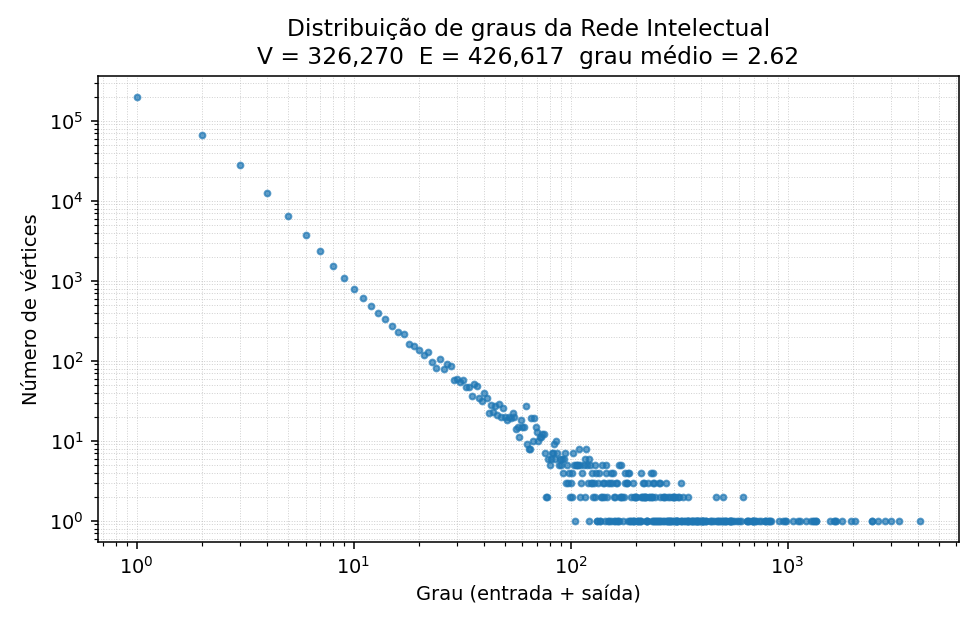
\includegraphics[width=0.78\linewidth]{grafico_distribuicao_graus.png}
  \caption{Distribuição do grau total em escala log-log. A maior parte dos vértices apresenta grau baixo, enquanto poucos hubs concentram grande número de relações.}
  \label{fig:graus}
\end{figure}

\subsection{Componentes fortemente conexas}

Uma componente fortemente conexa é um conjunto de vértices no qual cada vértice pode alcançar todos os demais respeitando a orientação das arestas. O grafo contém 325.240 componentes desse tipo, das quais 325.127 são unitárias. A maior componente possui 840 vértices.

A fragmentação é coerente com a semântica temporal e hierárquica de parte das relações. Arestas de orientação e influência tendem a seguir do orientador para o aluno ou de uma figura anterior para uma posterior, enquanto \texttt{almaMater} liga pessoas a instituições. Essas direções raramente formam caminhos de retorno, produzindo uma rede predominantemente acíclica. A consequência metodológica é relevante: algoritmos baseados em caminhadas aleatórias, principalmente quando executados em projeções restritas, podem alcançar somente uma parcela limitada do grafo a partir de determinada origem.

\begin{figure}[htbp]
  \centering
  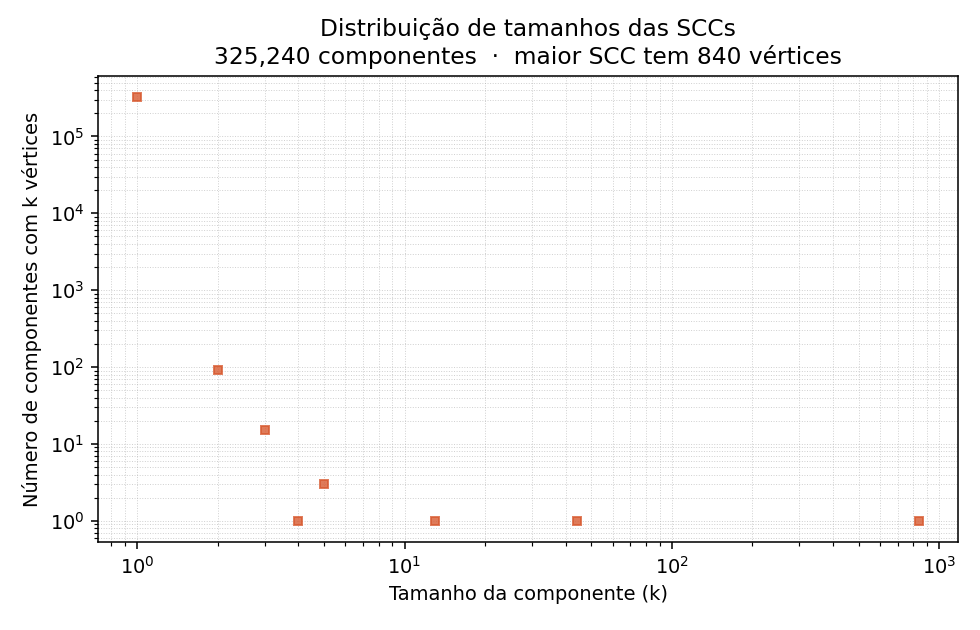
\includegraphics[width=0.78\linewidth]{grafico_distribuicao_componentes.png}
  \caption{Distribuição dos tamanhos das componentes fortemente conexas. Observa-se predominância de componentes unitárias e uma maior componente com 840 vértices.}
  \label{fig:componentes}
\end{figure}

\subsection{Visualização do núcleo estrutural}

Para produzir uma visualização legível, foi extraído um subgrafo em três etapas: seleção dos 500 vértices de maior grau no grafo completo, remoção dos vértices com grau inferior a 2 dentro desse subconjunto e escolha da maior componente fracamente conexa remanescente. O resultado contém 19 vértices e 60 arestas. A redução não foi utilizada no cálculo dos rankings; sua finalidade foi exclusivamente exploratória e visual.

O núcleo resultante é apresentado na Figura~\ref{fig:nucleo}, em conjunto com a amostra global produzida posteriormente no Neo4j Browser.

\section{Instanciação no Neo4j}

O grafo foi instanciado no Neo4j seguindo o modelo de grafo de propriedades. Cada recurso RDF foi representado por um nó com o rótulo \texttt{Resource} e duas propriedades principais: \texttt{uri}, que preserva seu identificador original, e \texttt{label}, que armazena uma forma legível do nome. Cada predicado foi convertido em um tipo de relacionamento em letras maiúsculas. Por exemplo,

\begin{lstlisting}
<http://dbpedia.org/resource/Albert_Einstein>
<http://dbpedia.org/ontology/influenced>
<http://dbpedia.org/resource/Niels_Bohr> .
\end{lstlisting}

é representado como:

\begin{lstlisting}
(Albert Einstein)-[:INFLUENCED]->(Niels Bohr)
\end{lstlisting}

O banco pode ser preparado de duas maneiras. Na primeira, utiliza-se o Neo4j Desktop: é possível criar uma instância vazia, instalar o plugin Graph Data Science e carregar o arquivo N-Triples com o script \texttt{neo4j/load\_graph.py}. O script lê as triplas em blocos, cria ou reutiliza nós e relacionamentos com \texttt{MERGE} e, ao final, cria índices sobre \texttt{Resource.uri} e \texttt{Resource.label}. Como opção mais rápida, o próprio Neo4j Desktop também permite criar uma instância a partir do dump previamente gerado, evitando a reinserção individual das 426.617 relações.

O mesmo dump pode ser utilizado pelo ambiente Docker, que o restaura automaticamente na primeira inicialização. A imagem Enterprise foi utilizada porque o dump está armazenado no formato \texttt{block}. O arquivo \texttt{compose.yaml} também instala os plugins APOC e Graph Data Science. Como o dump possui aproximadamente 325~MB e excede o limite de tamanho de arquivo do GitHub, ele foi disponibilizado em uma \href{https://drive.google.com/drive/folders/1s8zgb1wgWI-WAhUEZvB0qDljOAyWN4BZ?usp=sharing}{pasta externa no Google Drive}, acessível ao professor e aos autores do projeto.

Após a carga, o GDS cria projeções em memória com os tipos e orientações de relacionamentos definidos para cada experimento. Essas projeções não alteram a topologia armazenada no banco. Os escores calculados, entretanto, são gravados na propriedade \texttt{pageRank} dos vértices e exportados para arquivos TSV.

Como o Neo4j Browser renderiza no máximo 1.000 nós por padrão~\cite{neo4j-browser-settings}, não é possível representar simultaneamente os 326.270 vértices do grafo. A Figura~\ref{fig:neo4j-global} apresenta uma amostra global centrada nos 20 vértices de maior grau, limitada a 40 relações incidentes por vértice. A imagem não representa uma componente isolada nem a totalidade da rede; seu objetivo é mostrar a heterogeneidade dos principais hubs e de suas vizinhanças.

\begin{figure}[htbp]
  \centering
  \begin{subfigure}{0.48\linewidth}
    \centering
    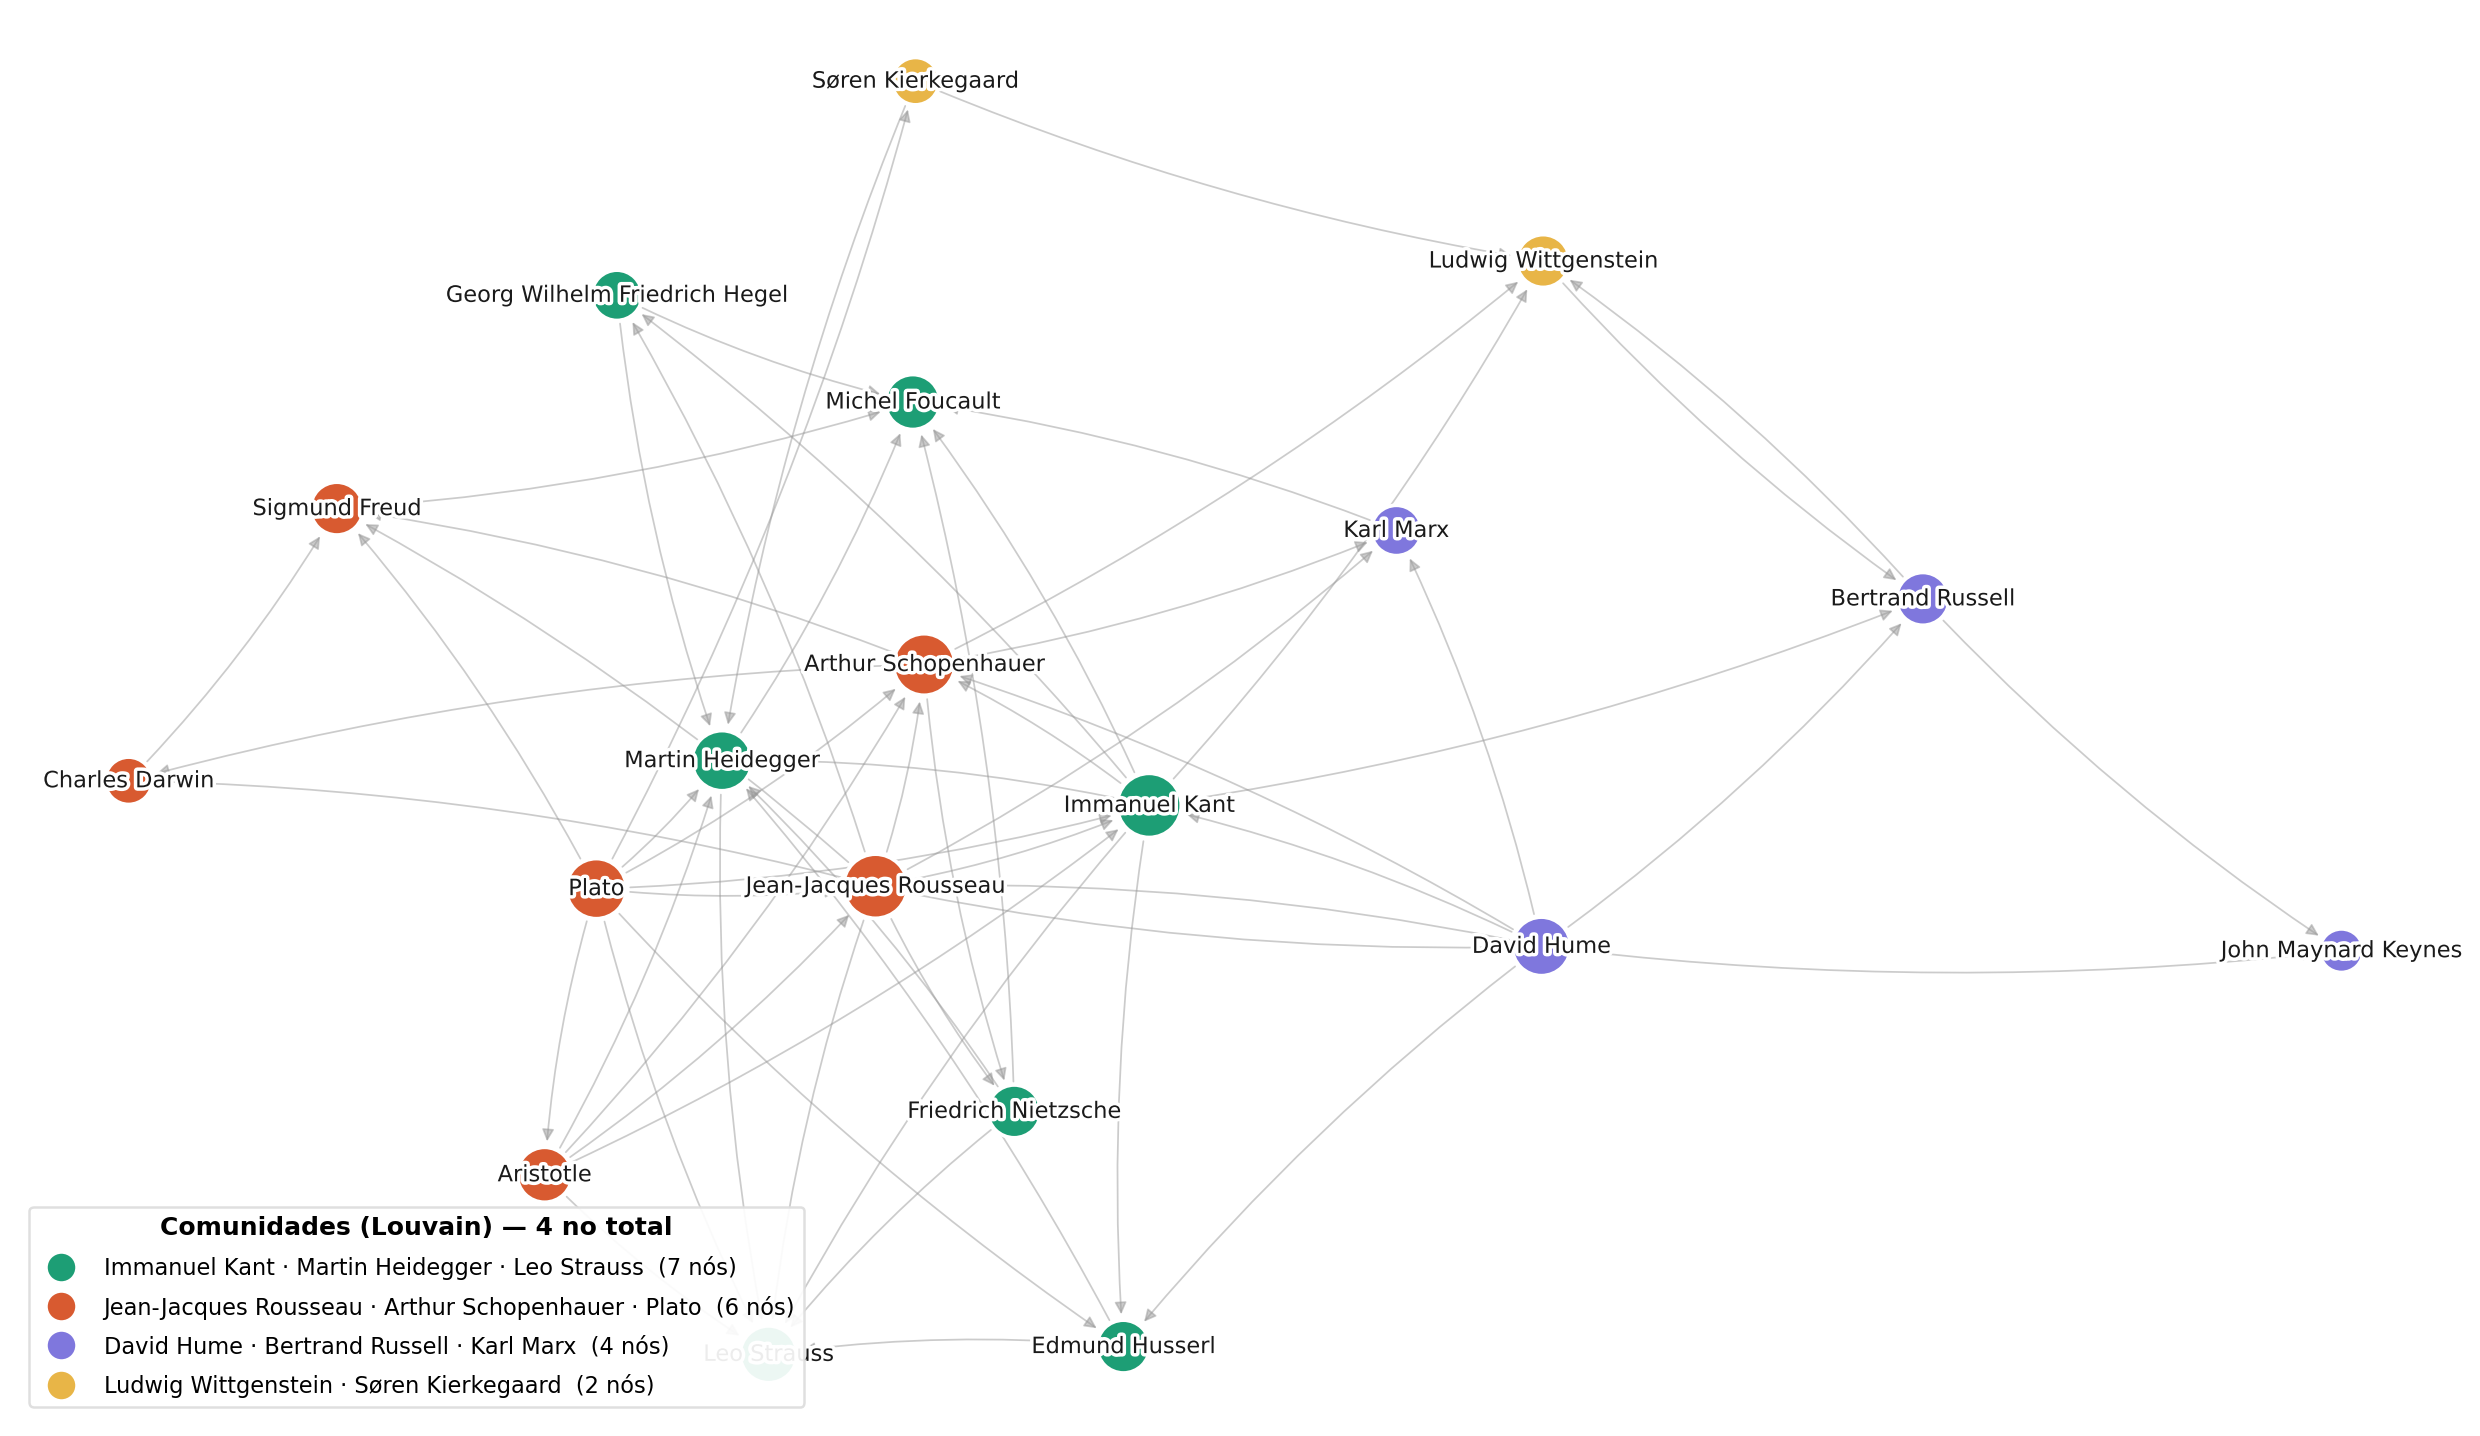
\includegraphics[width=\linewidth,height=0.25\textheight,keepaspectratio]{grafo_rede_intelectual.png}
    \caption{Núcleo estrutural com 19 vértices e 60 arestas.}
    \label{fig:nucleo}
  \end{subfigure}
  \hfill
  \begin{subfigure}{0.48\linewidth}
    \centering
    \includegraphics[width=\linewidth,height=0.25\textheight,keepaspectratio]{neo4j_visao_global.pdf}
    \caption{Amostra centrada nos 20 vértices de maior grau.}
    \label{fig:neo4j-global}
  \end{subfigure}
  \caption{Duas visualizações complementares da rede. Em (a), o núcleo denso usado na análise exploratória, com tamanho proporcional ao grau e cores definidas por Louvain. Em (b), a amostra global do Neo4j Browser, limitada a 40 relações incidentes por vértice e a no máximo 800 relações.}
  \label{fig:visoes-gerais}
\end{figure}

\section{PageRank}

\subsection{Fundamentação}

O PageRank foi proposto originalmente para estimar a importância de páginas da Web a partir da estrutura de hiperlinks~\cite{pagerank}. A ideia central é recursiva: um vértice recebe maior pontuação quando é apontado por vértices que também possuem alta pontuação. Em um grafo direcionado $G=(V,E)$, a atualização utilizada pode ser expressa por:

\begin{equation}
PR(v)=\frac{1-d}{|V|}
+d\sum_{u\in Pred(v)}\frac{PR(u)}{\operatorname{outdeg}(u)},
\label{eq:pagerank}
\end{equation}

onde $Pred(v)$ é o conjunto de predecessores de $v$, $\operatorname{outdeg}(u)$ é o grau de saída de $u$ e $d$ é o fator de amortecimento. O termo de teletransporte representa a possibilidade de abandonar a caminhada atual e reiniciá-la em outro vértice, reduzindo o efeito de sumidouros e ciclos fechados.

Os experimentos utilizaram a implementação do Neo4j GDS, com fator de amortecimento $d=0{,}85$ e limite de 20 iterações. Esses valores também correspondem aos padrões documentados pela biblioteca~\cite{neo4j-pagerank}. As arestas foram tratadas como não ponderadas. O GDS produz escores que não precisam somar 1; como a análise utiliza a ordem relativa, essa escala não altera os rankings.

\subsection{Pseudocódigo}

\begin{lstlisting}[caption={Pseudocódigo do PageRank iterativo.},label={lst:pagerank}]
função PageRank(Grafo G, real d, inteiro maxIterações):
    N <- quantidade de vértices de G

    para cada vértice v de G:
        PR[v] <- 1 / N

    para iteração <- 1 até maxIterações:
        para cada vértice v de G:
            novoPR[v] <- (1 - d) / N

        para cada vértice u de G:
            se grauSaída(u) > 0:
                parcela <- d * PR[u] / grauSaída(u)
                para cada vizinho de saída v de u:
                    novoPR[v] <- novoPR[v] + parcela
            senão:
                distribuir d * PR[u] / N entre todos os vértices

        PR <- novoPR

    retornar PR
\end{lstlisting}

Na execução efetiva, a iteração e o tratamento de vértices sem saída são realizados internamente por \texttt{gds.pageRank}. O script \texttt{neo4j/pagerank.py} é responsável por criar a projeção apropriada, executar o algoritmo, gravar os escores na propriedade \texttt{pageRank} e exportar o ranking para TSV.

\subsection{Projeções avaliadas}

O primeiro experimento executou o PageRank sobre o grafo completo, preservando a orientação natural das relações. Esperava-se encontrar, nas primeiras posições, figuras semelhantes às observadas no núcleo exploratório da Figura~\ref{fig:nucleo}, como Immanuel Kant, Leo Strauss e Karl Marx. O ranking obtido, entretanto, foi bastante diferente: além de instituições, religiões e áreas do conhecimento, sua primeira posição geral foi ocupada por Vaklush Tolev, figura búlgara associada à religião e à teologia~\cite{vaklush-dbpedia}, com escore 488,2684.

A investigação desse resultado mostrou que o PageRank não mede diretamente notoriedade histórica ou grau no núcleo visualizado. Ele modela um fluxo de prestígio que percorre as arestas na direção projetada, de modo que tanto o tipo quanto a orientação de uma relação determinam onde a pontuação se acumula. No subgrafo, Tolev recebe arestas \texttt{INFLUENCED} de oito tradições religiosas ou mitológicas. Entre elas, \textit{Islam} possui 3.004 arestas de entrada, PageRank 302,2443 e apenas uma aresta de saída; \textit{Christianity} possui 2.617 arestas de entrada, PageRank 223,9322 e também apenas uma saída. Como essas saídas apontam para Tolev, os dois vértices transferem a ele, respectivamente, cerca de 256,91 e 190,34 pontos após a aplicação do fator de amortecimento. Forma-se, assim, um funil no qual a centralidade acumulada por conceitos religiosos é quase integralmente direcionada a uma única pessoa.

Esse diagnóstico motivou a criação de projeções específicas e o teste da inversão das relações pessoais. Foram definidos três cenários para investigar o efeito da seleção e da orientação das arestas.

\textbf{Baseline.} A projeção inclui os nove tipos finais de relacionamento, em suas orientações naturais. Esse experimento mede centralidade global no grafo heterogêneo e serve como referência para as demais configurações.

\textbf{Pessoas.} A projeção inclui somente \texttt{INFLUENCED}, \texttt{DOCTORALSTUDENT} e \texttt{ACADEMICSTUDENT}, todos com orientação invertida pelo GDS. No arquivo final, essas relações apontam do mentor para o discípulo. Para o PageRank, porém, essa direção transfere pontuação ao discípulo. A inversão faz a caminhada seguir do discípulo para o mentor, permitindo interpretar o escore como prestígio recebido de pessoas influenciadas ou orientadas. No caso de Tolev, as arestas passam a sair dele em direção aos conceitos religiosos, eliminando o funil observado no baseline e aproximando o ranking da interpretação desejada de influência intelectual.

\textbf{Institucional.} A projeção inclui \texttt{INFLUENCED}, \texttt{DOCTORALSTUDENT}, \texttt{ACADEMICSTUDENT} e \texttt{ALMAMATER} em orientação natural. A relação \texttt{ALMAMATER} aponta da pessoa para a instituição; portanto, universidades acumulam prestígio proveniente de seus ex-alunos. As relações pessoais foram mantidas para preservar caminhos de influência e formação antes da transferência para as instituições.

\begin{table}[htbp]
  \centering
  \caption{Configuração dos experimentos de PageRank.}
  \label{tab:experimentos-pr}
  \begin{tabularx}{\linewidth}{lXl}
    \toprule
    Experimento & Relações & Orientação \\
    \midrule
    Baseline & Todos os nove tipos finais & Natural \\
    Pessoas & \texttt{INFLUENCED}, \texttt{DOCTORALSTUDENT}, \texttt{ACADEMICSTUDENT} & Invertida \\
    Institucional & As três relações anteriores e \texttt{ALMAMATER} & Natural \\
    \bottomrule
  \end{tabularx}
\end{table}

A Figura~\ref{fig:neo4j-segmentos} apresenta os três recortes utilizados para inspecionar visualmente os experimentos. As setas exibem a orientação armazenada no banco; no painel de pessoas, portanto, ainda não está aplicada a inversão realizada somente na projeção em memória do GDS.

\begin{figure}[htbp]
  \centering
  \begin{subfigure}{0.58\linewidth}
    \centering
    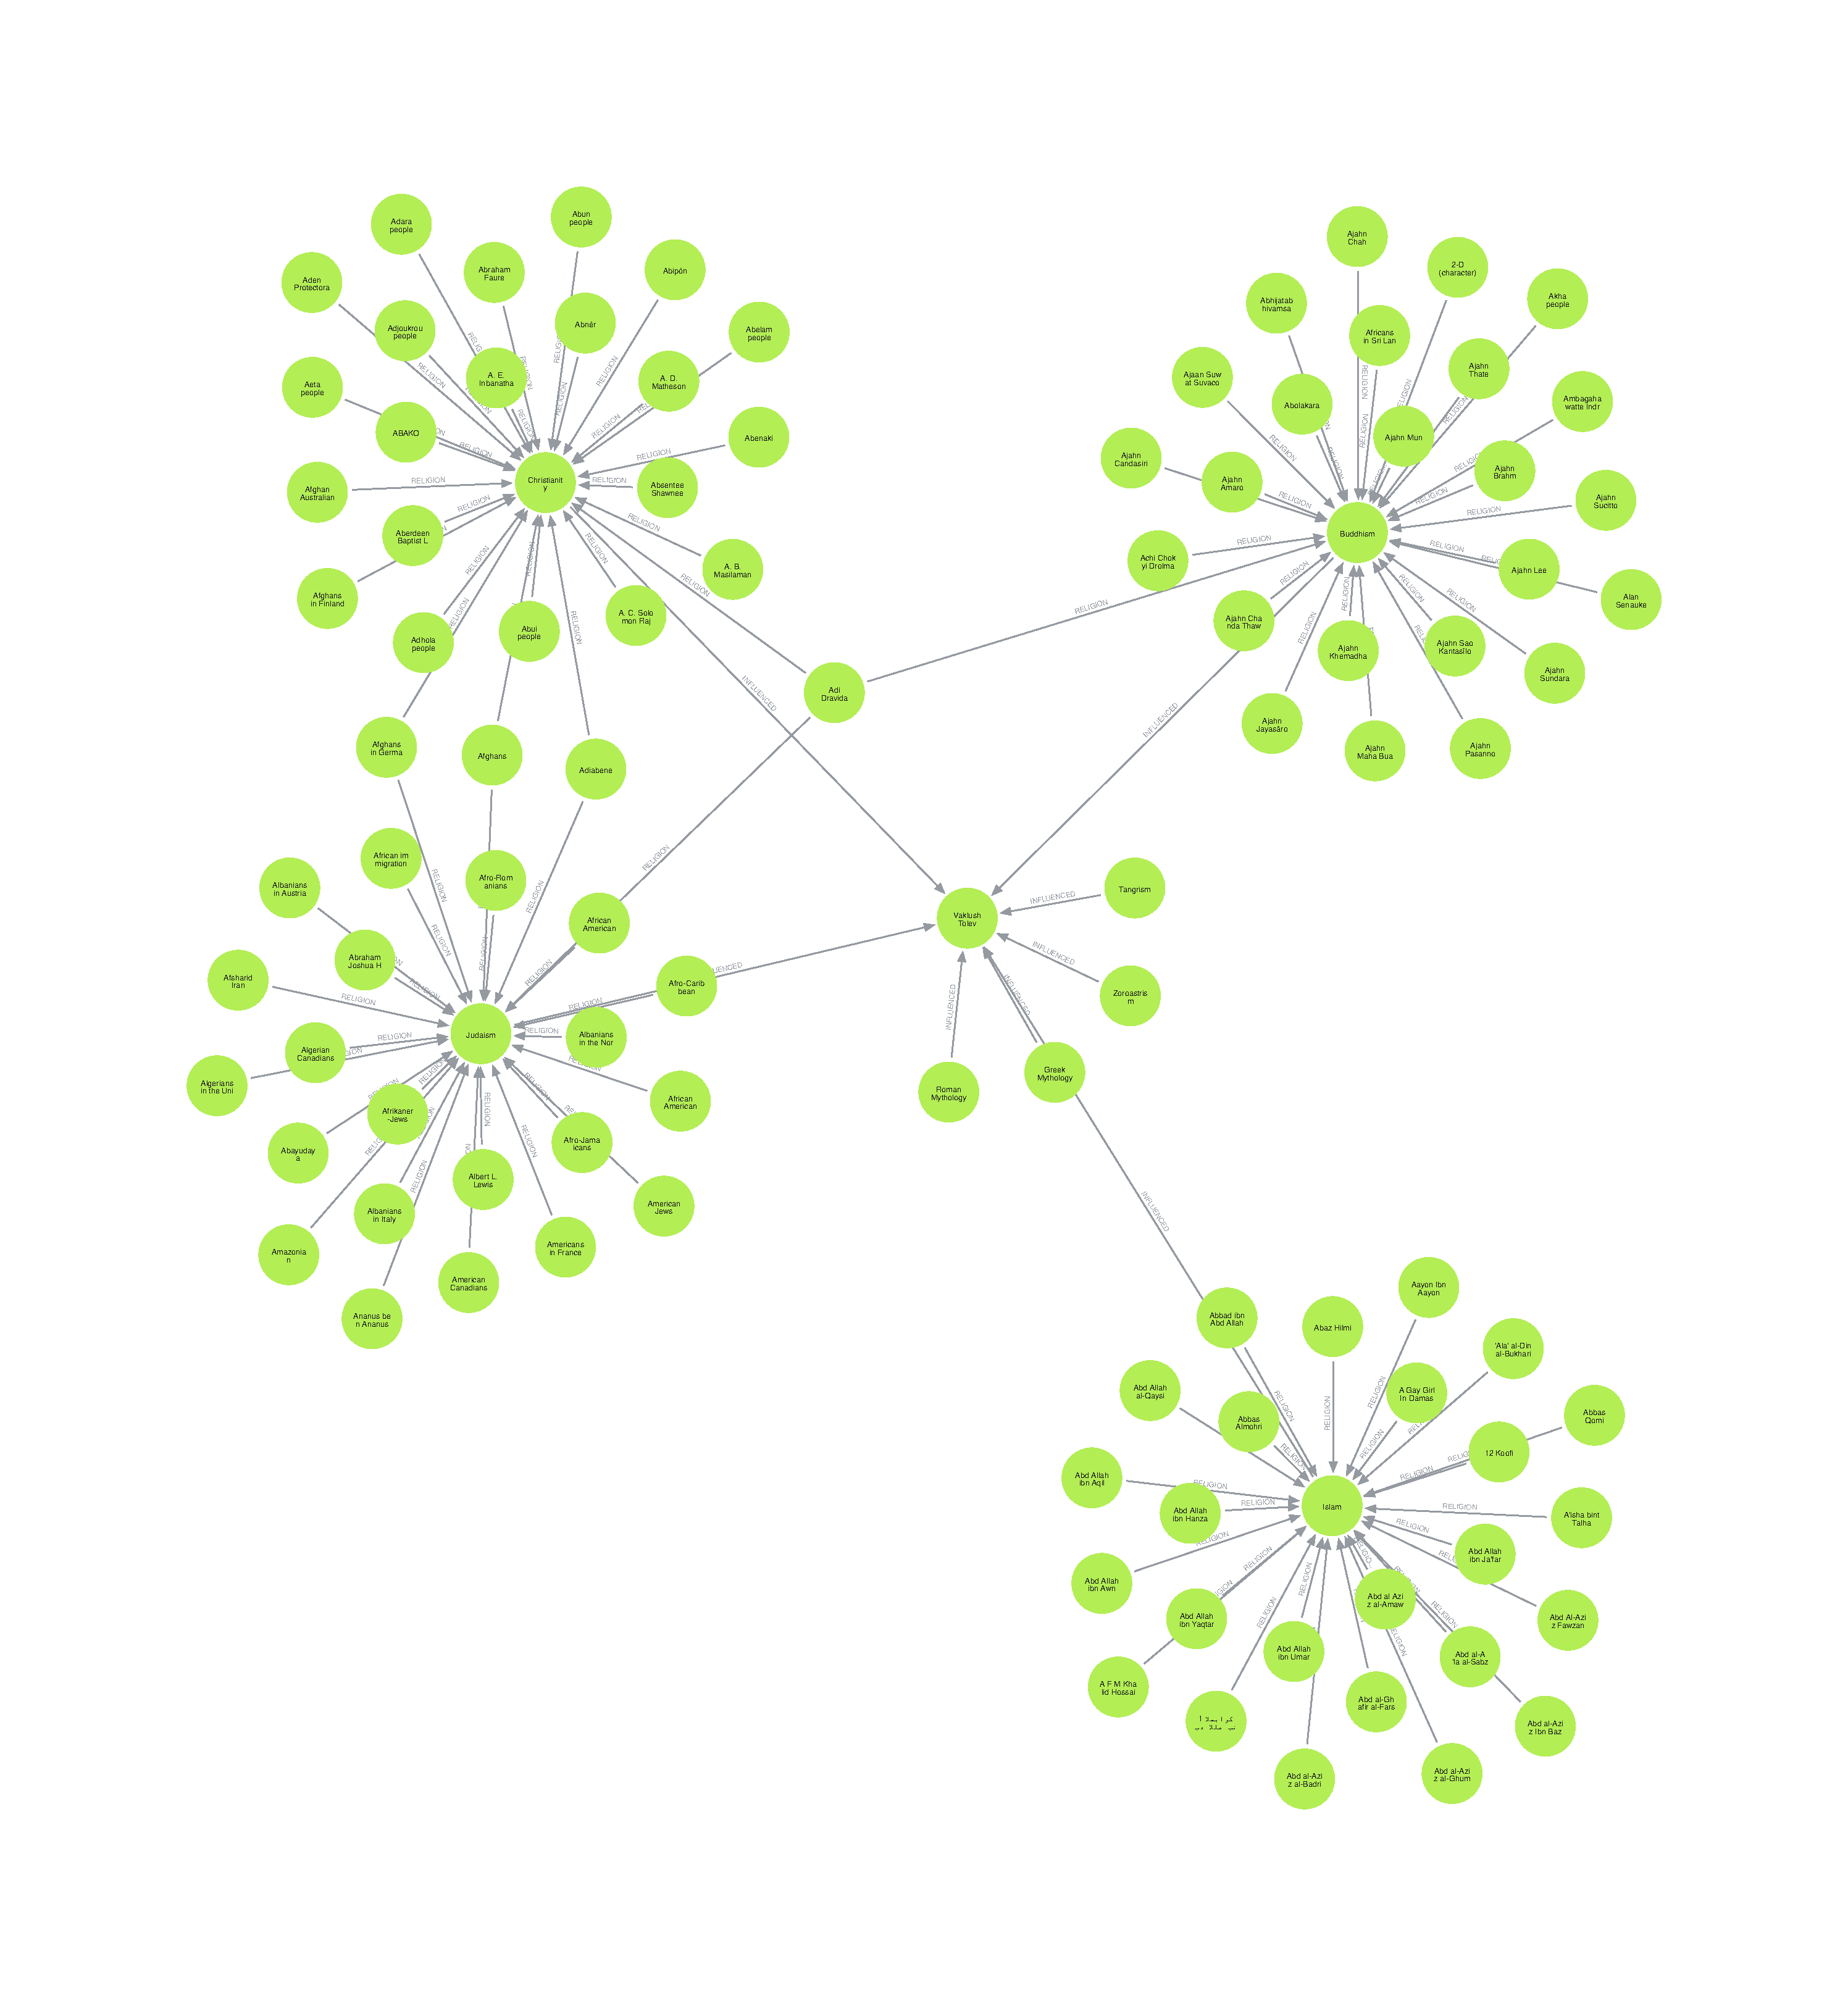
\includegraphics[width=\linewidth,height=0.30\textheight,keepaspectratio]{neo4j_funil_baseline.pdf}
    \caption{Funil do baseline em torno de Vaklush Tolev.}
    \label{fig:neo4j-funil}
  \end{subfigure}

  \begin{subfigure}{0.48\linewidth}
    \centering
    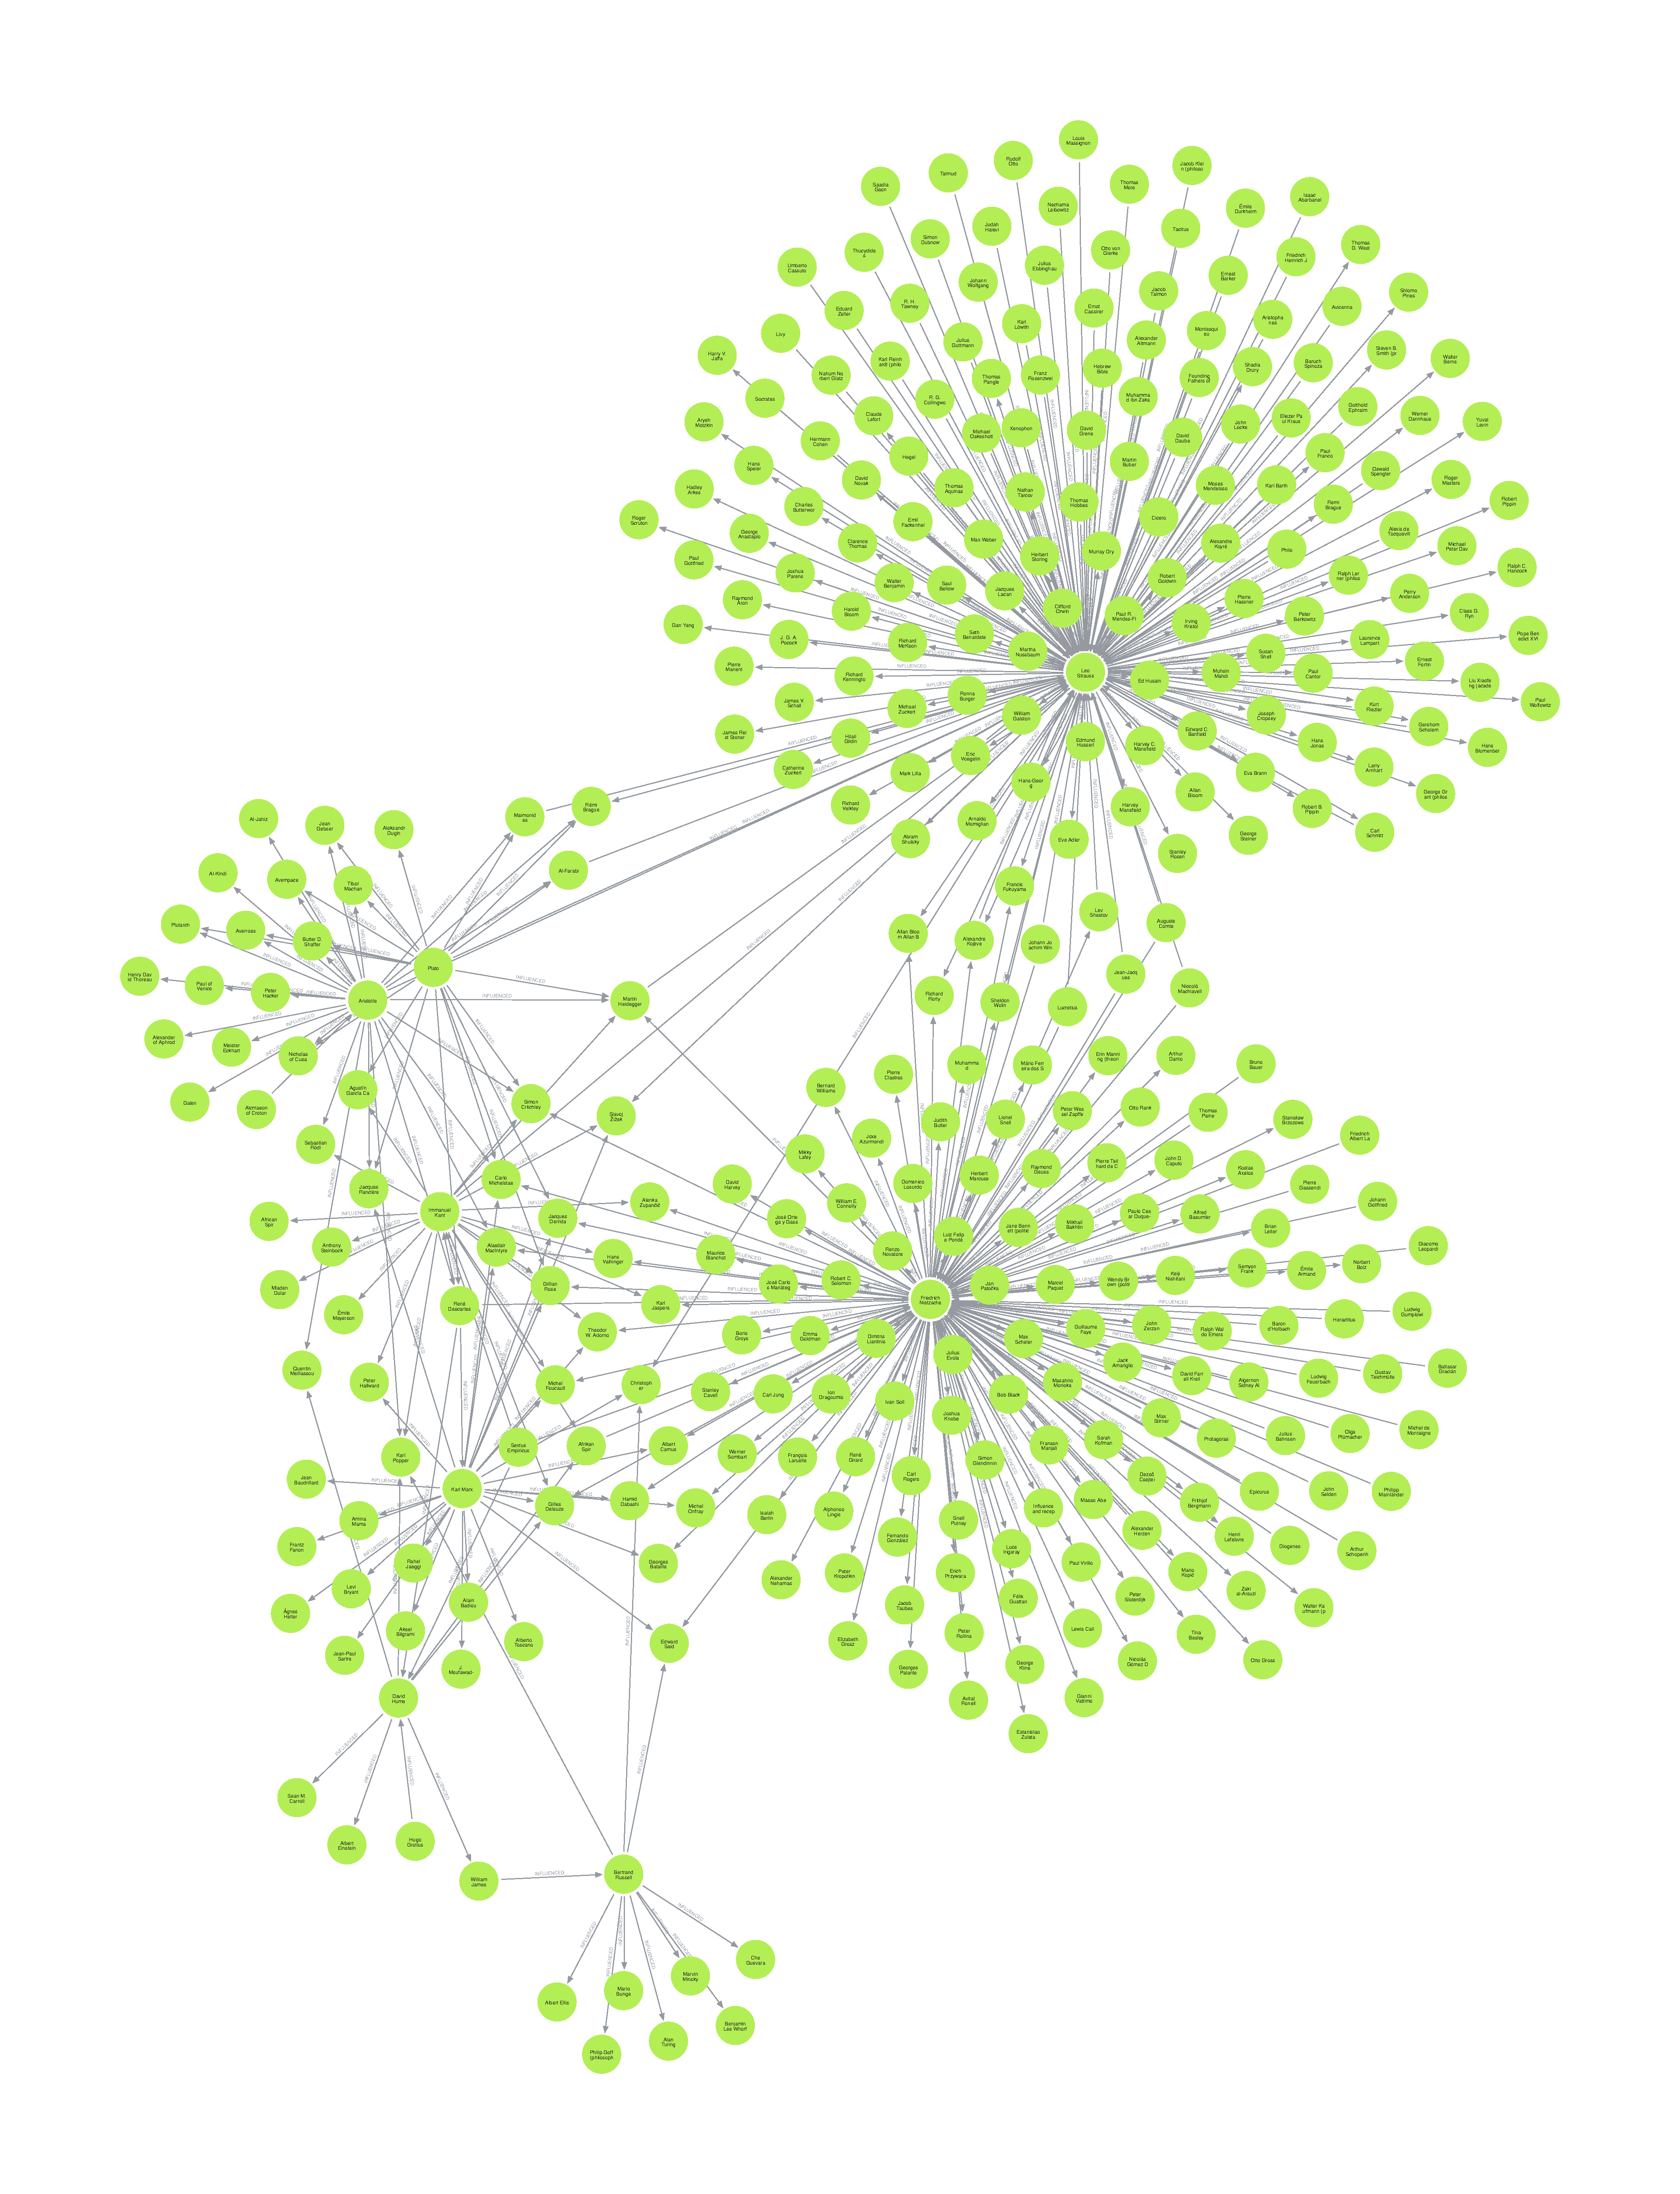
\includegraphics[width=\linewidth,height=0.26\textheight,keepaspectratio]{neo4j_segmento_pessoas.pdf}
    \caption{Relações de influência e orientação em torno de figuras do núcleo estrutural.}
    \label{fig:neo4j-pessoas}
  \end{subfigure}
  \hfill
  \begin{subfigure}{0.48\linewidth}
    \centering
    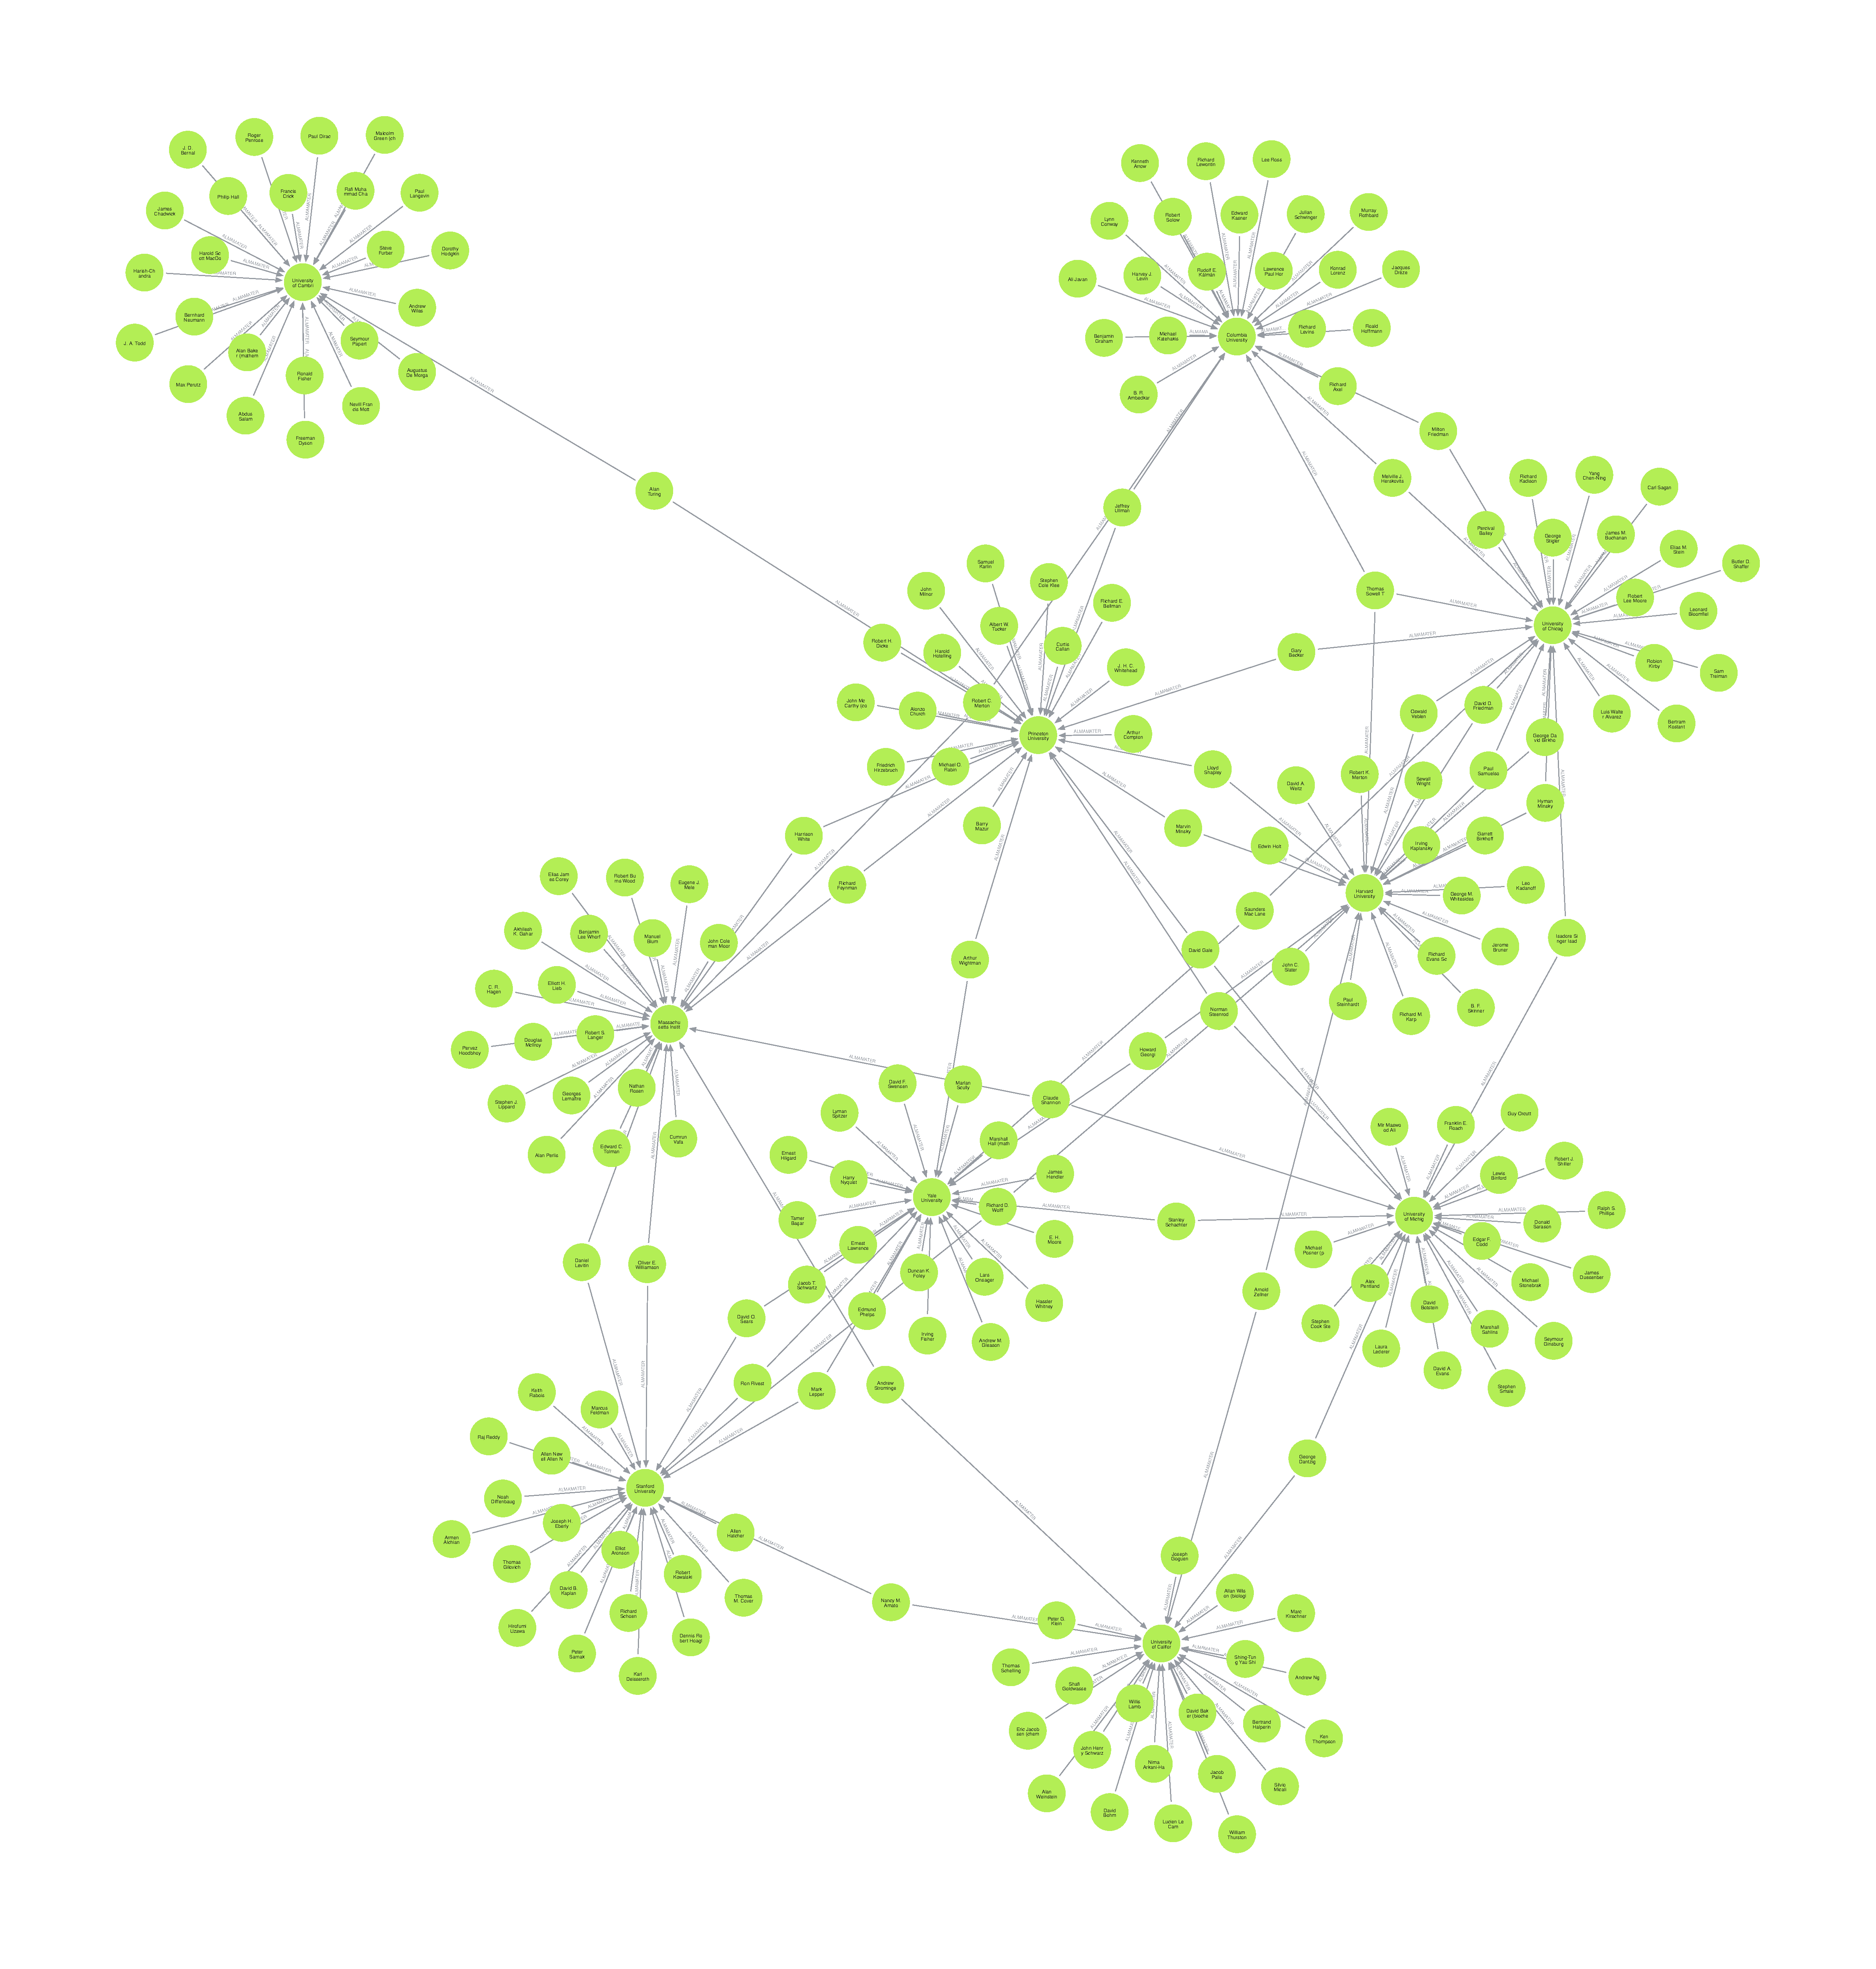
\includegraphics[width=\linewidth,height=0.26\textheight,keepaspectratio]{neo4j_segmento_institucional.pdf}
    \caption{Universidades selecionadas e seus ex-alunos de maior grau.}
    \label{fig:neo4j-institucional}
  \end{subfigure}
  \caption{Recortes do grafo produzidos no Neo4j Browser para examinar os três cenários de PageRank. Em (a), arestas \texttt{RELIGION} alimentam tradições que apontam para Tolev por \texttt{INFLUENCED}; em (b), são mostradas as direções originais das relações pessoais; em (c), \texttt{ALMAMATER} aponta dos ex-alunos para as instituições.}
  \label{fig:neo4j-segmentos}
\end{figure}

\section{Avaliação do PageRank}

\subsection{Referência para pessoas}

O ranking de pessoas foi comparado a uma referência construída a partir da Stanford Encyclopedia of Philosophy (SEP), enciclopédia acadêmica mantida pela Universidade Stanford~\cite{sep}. Inicialmente, o script \texttt{analysis/filter\_dbpedia\_people.py} consultou o endpoint SPARQL da DBpedia em lotes e manteve apenas recursos classificados como pessoa. As respostas foram armazenadas em cache para permitir a retomada do processo sem repetir consultas. Esse filtro produziu 3.936 candidatos válidos.

A referência externa foi construída pelo script \texttt{analysis/build\_sep\_citation\_ranking.py}, responsável pela raspagem automatizada das entradas da SEP. O programa parte da página de conteúdos da enciclopédia, coleta os endereços de todas as páginas sob \texttt{/entries/} e baixa seus documentos HTML. Para reduzir tráfego e tornar a execução retomável, cada página é armazenada em um cache local identificado pelo hash da URL; entre novos downloads, aplica-se ainda um intervalo de 0,5 segundo. A análise dos arquivos já armazenados é paralelizada entre os processadores disponíveis.

Antes do casamento dos nomes, o texto HTML é convertido para texto simples, com remoção de elementos de navegação, cabeçalhos, rodapés, scripts e estilos. Tanto o conteúdo quanto os rótulos dos candidatos passam por normalização Unicode, remoção de acentos e uniformização de espaços. O script também remove qualificadores finais de desambiguação, como ``\texttt{(philosopher)}'', e corrige rótulos com tokens repetidos. Para cada candidato, utiliza-se o nome completo como alias principal; o sobrenome é aceito como alias secundário somente quando é suficientemente longo, não corresponde a uma palavra comum e não aparece em outro candidato. Expressões regulares com limites de palavra evitam correspondências dentro de termos maiores.

Para cada candidato, contou-se em quantas entradas distintas da SEP ao menos um alias aparecia e quantas ocorrências brutas foram encontradas. O primeiro valor foi adotado como escore de referência, pois reduz o peso de repetições dentro de uma mesma página; a contagem bruta serviu como critério secundário de desempate. O arquivo resultante, \texttt{analysis/sep\_citation\_ranking.tsv}, também registra os aliases reconhecidos e até cinco exemplos de páginas correspondentes, permitindo auditar os resultados da raspagem.

Foram empregadas duas métricas. A correlação de Spearman compara a ordem dos candidatos comuns aos dois rankings. Já o Overlap@$k$ mede a fração de elementos compartilhados entre os $k$ primeiros colocados do PageRank e da referência da SEP:

\begin{equation}
Overlap@k=\frac{|Top_k(PR)\cap Top_k(SEP)|}{k}.
\end{equation}

O uso de Overlap@$k$ decorre da natureza simétrica dessa comparação: tanto o PageRank quanto a SEP produzem rankings, e a pergunta é quanto seus respectivos conjuntos Top-$k$ concordam. A SEP não é tratada como uma lista absoluta de respostas corretas, mas como uma ordenação externa com a qual se deseja medir concordância.

Essa referência não deve ser interpretada como medida absoluta de importância filosófica. A frequência de nomes na SEP depende de cobertura editorial, ambiguidades e do papel desempenhado por certos autores na própria enciclopédia. Ela fornece, contudo, um critério externo reproduzível para comparar as duas projeções do mesmo grafo.

\subsection{Referência para universidades}

As universidades foram identificadas por palavras-chave em seus rótulos, como \texttt{university}, \texttt{college}, \texttt{polytechnic} e equivalentes em outros idiomas. Os resultados foram comparados ao Top 20 do Center for World University Rankings (CWUR) de 2026~\cite{cwur2026}. Diferentemente da comparação entre pessoas, o Top 20 do CWUR foi tratado como um conjunto fixo de instituições relevantes. A Precision@$k$ corresponde, portanto, à proporção das $k$ universidades mais bem colocadas pelo PageRank que pertencem a esse conjunto de elite:

\begin{equation}
Precision@k=\frac{|Top_k(PR)\cap Elite_{CWUR}|}{k}.
\end{equation}

Essa métrica responde quantas das instituições recomendadas pelo algoritmo são consideradas relevantes pela referência. Por exemplo, Precision@10 igual a 100\% significa que todas as dez primeiras universidades do PageRank pertencem ao Top 20 do CWUR; não significa que as vinte instituições da referência tenham sido recuperadas. A correlação de Spearman foi calculada separadamente entre as posições das universidades do CWUR encontradas no grafo.

O CWUR avalia universidades por critérios diferentes da centralidade desta rede e, por isso, funciona como referência aproximada, não como verdade fundamental. A comparação verifica se as relações de formação e influência recuperam instituições reconhecidas externamente.

\section{Resultados e discussão do PageRank}

\subsection{Pessoas e intelectuais}

A projeção reversa para pessoas apresentou resultados superiores ao baseline em todas as métricas. A correlação de Spearman aumentou de 0,230920 para 0,499841. O Overlap@20 passou de 0\% para 35\%, e o Overlap@50 passou de 4\% para 40\%.

\begin{table}[htbp]
  \centering
  \caption{PageRank de pessoas comparado à referência da SEP.}
  \label{tab:resultado-pessoas}
  \begin{tabular}{lrrr}
    \toprule
    Projeção & Spearman & Overlap@20 & Overlap@50 \\
    \midrule
    Baseline & 0,230920 & 0\% & 4\% \\
    Pessoas, relações invertidas & \textbf{0,499841} & \textbf{35\%} & \textbf{40\%} \\
    \bottomrule
  \end{tabular}
\end{table}

\begin{table}[htbp]
  \centering
  \caption{Dez primeiros candidatos válidos na projeção de pessoas.}
  \label{tab:top-pessoas}
  \begin{tabular}{r l r}
    \toprule
    Posição & Pessoa & Escore \\
    \midrule
    1 & Immanuel Kant & 58,0966 \\
    2 & Aristotle & 50,1809 \\
    3 & Plato & 40,7841 \\
    4 & Gottfried Wilhelm Leibniz & 27,3950 \\
    5 & Pythagoras & 27,2734 \\
    6 & Ferdinand von Lindemann & 25,6811 \\
    7 & Parmenides & 23,4694 \\
    8 & Heraclitus & 23,0318 \\
    9 & Bertrand Russell & 20,3374 \\
    10 & David Hume & 19,7355 \\
    \bottomrule
  \end{tabular}
\end{table}

O ganho confirma que a orientação semântica das arestas é decisiva. No baseline, relações heterogêneas fazem a pontuação fluir para instituições, religiões, áreas e obras. Na projeção de pessoas, a remoção dessas relações reduz a competição com entidades que não são indivíduos, enquanto a inversão direciona prestígio de discípulos para mentores. Kant, Aristóteles e Platão passam a ocupar as primeiras posições, em maior concordância com a referência externa.

A correlação permanece abaixo de uma concordância perfeita. Isso é esperado porque os critérios não são equivalentes: o PageRank mede posição estrutural nas relações registradas pela DBpedia, enquanto a referência mede presença textual nas entradas da SEP. O aparecimento de Ferdinand von Lindemann entre os dez primeiros, por exemplo, indica que cadeias acadêmicas muito documentadas podem elevar candidatos cuja presença na tradição filosófica é mais restrita. Esse caso evidencia tanto a informação capturada pelo grafo quanto o viés de cobertura de suas relações.

\subsection{Universidades}

Para universidades, o baseline obteve Precision@10 de 100\%, enquanto a projeção institucional atingiu 90\%. Ambas alcançaram Precision@20 de 65\%. A correlação com a ordem do CWUR também foi ligeiramente maior no baseline: 0,545865 contra 0,526316.

\begin{table}[htbp]
  \centering
  \caption{PageRank de universidades comparado ao CWUR 2026.}
  \label{tab:resultado-universidades}
  \begin{tabular}{lrrr}
    \toprule
    Projeção & Precision@10 & Precision@20 & Spearman \\
    \midrule
    Baseline & \textbf{100\%} & 65\% & \textbf{0,545865} \\
    Institucional & 90\% & 65\% & 0,526316 \\
    \bottomrule
  \end{tabular}
\end{table}

\begin{table}[htbp]
  \centering
  \caption{Dez primeiras universidades na projeção institucional.}
  \label{tab:top-universidades}
  \begin{tabular}{r l r}
    \toprule
    Posição & Universidade & Escore \\
    \midrule
    1 & Harvard University & 318,0176 \\
    2 & University of Michigan & 288,3303 \\
    3 & Princeton University & 244,0913 \\
    4 & Yale University & 220,1037 \\
    5 & Columbia University & 189,7218 \\
    6 & University of Chicago & 146,7403 \\
    7 & University of Cambridge & 141,6175 \\
    8 & University of California, Berkeley & 138,6354 \\
    9 & Stanford University & 135,5410 \\
    10 & Hebrew University of Jerusalem & 129,1625 \\
    \bottomrule
  \end{tabular}
\end{table}

A projeção institucional concentrou as primeiras posições em universidades reconhecidas, demonstrando que \texttt{ALMAMATER} oferece um sinal relevante de prestígio. Entretanto, ela não superou o baseline segundo as métricas adotadas. Isso sugere que as demais relações do grafo completo também carregam informação útil para instituições ou que a composição institucional escolhida ainda preserva ruído suficiente para alterar as primeiras posições.

Os resultados mostram que uma projeção especializada não é automaticamente superior. No caso de pessoas, a direção original contrariava o fluxo de prestígio desejado e sua inversão produziu ganho expressivo. No caso institucional, \texttt{ALMAMATER} já possuía a direção adequada, e a restrição do conjunto de relações não trouxe melhora mensurável. A seleção das arestas deve, portanto, ser fundamentada na semântica de cada relação e validada empiricamente.

\section{Personalized PageRank e predição de ligações}

\subsection{Motivação e formulação}

O Personalized PageRank (PPR) modifica o mecanismo de teletransporte do PageRank. Em vez de reiniciar a caminhada aleatória uniformemente em qualquer vértice, concentra-se a probabilidade de reinício em um vértice fonte $s$. Seja $P$ a matriz de transição do grafo, $\mathbf{e}_s$ o vetor que vale 1 em $s$ e 0 nos demais vértices e $d$ o fator de amortecimento. O vetor personalizado é obtido iterativamente por

\begin{equation}
\boldsymbol{\pi}_s^{(i+1)}=(1-d)\mathbf{e}_s+dP^{\mathsf{T}}\boldsymbol{\pi}_s^{(i)}.
\label{eq:ppr}
\end{equation}

Valores elevados de $\pi_s(t)$ indicam que $t$ é estruturalmente alcançável e relevante a partir de $s$. O PPR não avalia diretamente o significado textual das entidades: ele mede proximidade topológica condicionada à orientação e aos tipos de aresta. Por essa razão, a comparação com similaridade lexical da WordNet, prevista na proposta inicial, foi substituída por uma avaliação de predição de ligações. Esse protocolo testa diretamente se a estrutura conhecida é capaz de recuperar relações reais deliberadamente ocultadas.

\subsection{Construção dos conjuntos de treino e teste}

O script \texttt{neo4j/split\_edges.py} parte das 426.617 arestas e calcula iterativamente o núcleo de ordem 5 do grafo não direcionado subjacente. Permanecem nesse núcleo 2.698 vértices e 14.233 arestas. O filtro é usado apenas para definir quais arestas podem ser ocultadas; as regiões periféricas continuam disponíveis no grafo de treino.

Com semente pseudoaleatória 42, selecionam-se 10\% das arestas elegíveis, resultando em 1.423 casos de teste. Uma aresta $(s,r,t)$ só pode ser removida se, após sua retirada, a origem mantiver ao menos duas saídas, o destino mantiver ao menos uma entrada e ambos preservarem grau total mínimo 3 dentro do núcleo. Essas restrições evitam casos triviais em que a própria ocultação isola os vértices avaliados.

As arestas escolhidas são registradas em \texttt{neo4j/test\_edges.tsv}, marcadas temporariamente no banco e então removidas fisicamente. O grafo restante constitui $G_{treino}$ e o TSV funciona como gabarito $E_{teste}$. Como as ligações avaliadas não participam das projeções do GDS, o algoritmo não pode utilizar a resposta durante o cálculo, prevenindo vazamento de dados.

\subsection{Execução do PPR}

O script \texttt{neo4j/ppr.py} agrupa as arestas de teste por tipo de relação. Para cada tipo $r$, cria-se uma projeção GDS contendo somente relações desse tipo em orientação natural. Em seguida, para cada origem distinta $s$ presente no gabarito, executa-se \texttt{gds.pageRank.stream} com $s$ como \texttt{sourceNode}, fator de amortecimento 0,85, limite de 20 iterações e retenção dos 500 destinos de maior escore, excluindo a própria origem. As fontes são processadas em lotes de 50 e cada projeção é descartada após o término do respectivo tipo, reduzindo o consumo de memória.

Para uma aresta oculta $(s,r,t)$, o ranking produzido a partir de $(s,r)$ é interpretado como uma lista de destinos candidatos. A predição é considerada recuperada quando $t$ aparece nessa lista. O procedimento completo é sintetizado no pseudocódigo a seguir.

\begin{lstlisting}[caption={Pseudocódigo da avaliação do PPR por predição de ligações.},label={lst:ppr}]
função AvaliarPPR(G, k=5, proporçãoTeste=0.10, K=500):
    C <- k-core de ordem k do grafo subjacente de G
    E_teste <- selecionar arestas de C preservando graus mínimos
    G_treino <- G sem E_teste

    para cada tipo de relação r presente em E_teste:
        G_r <- projetar em G_treino somente as relações do tipo r

        para cada origem distinta s das arestas (s, r, t):
            ranking[s, r] <- Top-K do PPR(G_r, fonte=s)

        descartar G_r

    para cada aresta (s, r, t) em E_teste:
        rank[s, r, t] <- posição de t em ranking[s, r]

    retornar HitRate@K, MRR e recuperação no Top-500
\end{lstlisting}

\subsection{Métricas}

O HitRate@$k$ mede a proporção de arestas ocultadas cujo destino verdadeiro aparece entre os $k$ primeiros candidatos. Para cada caso há um destino de teste específico; por isso, HitRate é mais apropriado que Precision, que dividiria o número de itens relevantes recuperados pelo total de $k$ recomendações:

\begin{equation}
HitRate@k=\frac{1}{|E_{teste}|}
\sum_{(s,r,t)\in E_{teste}}
\mathbb{1}\!\left[t\in Top_k(s,r)\right].
\label{eq:hitrate}
\end{equation}

O Mean Reciprocal Rank (MRR) considera também a posição do destino correto. Acertos nas primeiras posições recebem maior peso, enquanto arestas não recuperadas contribuem com zero:

\begin{equation}
MRR=\frac{1}{|E_{teste}|}
\sum_{(s,r,t)\in E_{teste}}
\begin{cases}
1/\operatorname{rank}_{s,r}(t), & \text{se }t\text{ foi recuperado};\\
0, & \text{caso contrário}.
\end{cases}
\label{eq:mrr}
\end{equation}

O código denomina \textit{coverage} a fração de arestas encontradas no Top-500. No relatório, essa medida é chamada de taxa de recuperação no Top-500 para distingui-la da noção tradicional de cobertura de usuários ou itens em sistemas de recomendação.

\subsection{Resultados e interpretação}

As métricas foram recalculadas diretamente a partir das 1.423 linhas do artefato final \path{neo4j/ppr_predictions.tsv}. O PPR recuperou 439 destinos no Top-500, equivalentes a 30,85\% do conjunto de teste. Entretanto, apenas 4,22\% das arestas apareceram nas vinte primeiras posições, e o MRR foi 0,011418. A Tabela~\ref{tab:ppr-resultados} resume os resultados.

\begin{table}[htbp]
  \centering
  \caption{Resultados do PPR na tarefa de predição de ligações.}
  \label{tab:ppr-resultados}
  \begin{tabular}{lr@{\qquad}lr}
    \toprule
    Métrica & Valor & Métrica & Valor \\
    \midrule
    Arestas de teste & 1.423 & Recuperadas no Top-500 & 439 (30,85\%) \\
    HitRate@1 & 0,002811 & HitRate@5 & 0,011947 \\
    HitRate@10 & 0,021082 & HitRate@20 & 0,042164 \\
    MRR & 0,011418 & & \\
    \bottomrule
  \end{tabular}
\end{table}

O desempenho varia fortemente entre os tipos de relacionamento. Das 736 arestas \texttt{INFLUENCED} avaliadas, 436 foram encontradas no Top-500, uma taxa de 59,24\%. Para \texttt{IDEOLOGY}, houve 3 acertos em 462 casos; nos demais 225 casos, distribuídos entre \texttt{RELIGION}, \texttt{ALMAMATER}, \texttt{FIELD}, \texttt{DOCTORALSTUDENT}, \texttt{ACADEMICSTUDENT} e \texttt{KNOWNFOR}, não houve recuperação.

Essa diferença é explicada pela topologia das projeções. \texttt{INFLUENCED} forma cadeias direcionadas nas quais pessoas podem atuar simultaneamente como origem e destino, oferecendo caminhos alternativos até uma ligação ocultada. Relações como \texttt{ALMAMATER}, \texttt{RELIGION} e \texttt{FIELD} são predominantemente bipartidas: pessoas apontam para instituições, religiões ou áreas que raramente possuem saídas do mesmo tipo. Quando a aresta direta é removida, o destino tende a se tornar inalcançável naquela projeção. Assim, a taxa global de 30,85\% é concentrada quase inteiramente na rede de influência.

Os valores baixos de HitRate nos primeiros cortes e de MRR mostram ainda que muitos dos destinos recuperados aparecem longe do topo. O experimento confirma que o PPR captura proximidade estrutural quando existem caminhos direcionados alternativos, mas não substitui informação semântica ausente. Projeções não direcionadas, combinações de diferentes tipos de relação ou pesos específicos poderiam ampliar a conectividade, porém constituiriam hipóteses distintas e exigiriam nova validação para evitar que o ganho decorresse apenas da introdução artificial de caminhos.

\section{Uso de inteligência artificial generativa}

Ferramentas de IA generativa foram utilizadas como apoio à análise exploratória, à programação, à infraestrutura e à redação técnica. Nos estágios iniciais, elas auxiliaram a inspecionar o dump da DBpedia, que contém milhões de triplas, e a identificar predicados e padrões compatíveis com o recorte intelectual proposto. Também apoiaram a elaboração e a revisão dos scripts de filtragem, cálculo de métricas, raspagem da SEP, consultas Cypher e automação do ambiente com Docker Compose.

O Antigravity foi empregado principalmente como copiloto de infraestrutura. A ferramenta auxiliou no diagnóstico de conflitos entre o Neo4j Desktop e o Docker, incluindo portas ocupadas, volumes bloqueados, permissões de arquivos e problemas de DNS e IPv6 na JVM. Também apoiou a identificação da incompatibilidade entre o formato \texttt{block} do dump e a edição Community, a migração da composição para Neo4j Enterprise e a criação do \texttt{load\_dump.sh}, responsável por restaurar automaticamente o banco sem sobrescrever volumes já inicializados.

O Codex, da OpenAI, foi utilizado para inspecionar o repositório e cruzar documentação, código e artefatos; formalizar as métricas e os pseudocódigos; revisar a interpretação dos experimentos; elaborar consultas Cypher para as visualizações; estruturar o relatório em LaTeX e verificar sua compilação e paginação. Em particular, a ferramenta ajudou a detectar divergências entre execuções do PPR, razão pela qual as métricas finais foram recalculadas diretamente a partir do TSV de predições.

Todas as sugestões foram avaliadas pelos autores. A definição do problema, a escolha dos dados e experimentos, a execução dos programas, a inspeção dos resultados e a decisão de aceitar, modificar ou rejeitar cada proposta permaneceram sob responsabilidade de Raphael Salles Vitor de Souza e Lucas Félix. Os valores apresentados no relatório foram produzidos pelos scripts e artefatos do projeto, e não estimados pelos modelos generativos.

\section{Conclusão}

Este trabalho transformou um dump de 22,8 milhões de triplas da DBpedia em uma rede intelectual direcionada, reproduzível e adequada à análise em Neo4j. A seleção e a normalização de 11 predicados resultaram em 326.270 vértices e 426.617 arestas. A rede apresentou forte heterogeneidade de graus e elevada fragmentação dirigida: 99,97\% das componentes fortemente conexas são unitárias. Essas propriedades não são apenas descritivas, pois condicionam diretamente o funcionamento dos algoritmos de caminhada aleatória.

Os experimentos de PageRank mostraram que a semântica e a orientação das arestas são determinantes. A projeção invertida de pessoas elevou a correlação de Spearman com a SEP de 0,230920 para 0,499841 e o Overlap@50 de 4\% para 40\%. Já a projeção institucional não superou o baseline, indicando que restringir relações não garante melhoria automática. O caso de Vaklush Tolev evidenciou como hubs religiosos e arestas orientadas podem criar funis de prestígio inesperados.

Na predição de ligações, o PPR recuperou 30,85\% das arestas ocultadas no Top-500, mas obteve HitRate@20 de apenas 4,22\% e MRR de 0,011418. Quase todos os acertos vieram de \texttt{INFLUENCED}, cuja topologia oferece caminhos alternativos; relações bipartidas, como \texttt{ALMAMATER} e \texttt{RELIGION}, tornaram seus destinos inalcançáveis após a ocultação da ligação direta. Conclui-se que a topologia contém sinal útil de influência, mas proximidade estrutural e proximidade semântica não são equivalentes. Trabalhos futuros podem investigar projeções heterogêneas ponderadas, informação textual e validações temporais, preservando um protocolo sem vazamento de dados.

\clearpage
\appendix
\section{Consultas Cypher das visualizações}

As consultas a seguir foram executadas no Neo4j Browser para produzir os SVGs das Figuras~\ref{fig:neo4j-global} e~\ref{fig:neo4j-segmentos}. Os limites fazem parte do protocolo de visualização e evitam ultrapassar a capacidade de renderização da ferramenta. O arquivo executável completo está disponível em \texttt{docs/latex/neo4j\_visualizations.cypher}.

\lstinputlisting[
  firstline=1,
  lastline=20,
  basicstyle=\ttfamily\tiny,
  numbers=left,
  numberstyle=\tiny,
  caption={Consulta da amostra global representativa.},
  label={lst:neo4j-global}
]{neo4j_visualizations.cypher}

\lstinputlisting[
  firstline=23,
  lastline=40,
  basicstyle=\ttfamily\tiny,
  numbers=left,
  numberstyle=\tiny,
  caption={Consulta do funil do baseline em torno de Vaklush Tolev.},
  label={lst:neo4j-funil}
]{neo4j_visualizations.cypher}

\lstinputlisting[
  firstline=43,
  lastline=66,
  basicstyle=\ttfamily\tiny,
  numbers=left,
  numberstyle=\tiny,
  caption={Consulta do segmento de pessoas.},
  label={lst:neo4j-pessoas}
]{neo4j_visualizations.cypher}

\lstinputlisting[
  firstline=69,
  lastline=97,
  basicstyle=\ttfamily\tiny,
  numbers=left,
  numberstyle=\tiny,
  caption={Consulta do segmento institucional.},
  label={lst:neo4j-institucional}
]{neo4j_visualizations.cypher}

\printbibliography[title={Referências}]

\end{document}
